\chapter{Motivation}
\label{motivation}

Consensus is a fundamental problem in fault-tolerant systems: how can
servers reach agreement on shared state, even in the face of failures?
This problem arises in a wide variety of systems that need to provide
high levels of availability and cannot compromise on consistency; thus,
consensus is used in virtually all consistent large-scale storage
systems. Section~\ref{motivation:problem} describes how consensus is
typically used to create replicated state machines, a general-purpose
building block for fault-tolerant systems; Section~\ref{motivation:uses}
discusses various ways replicated state machines are used in larger
systems; and Section~\ref{motivation:paxos} discusses the problems with
the Paxos consensus protocol, which Raft aims to address.

\section{Achieving fault tolerance with replicated state machines}
\label{motivation:problem}

Consensus algorithms typically arise in the context of
\emph{replicated state machines}~\cite{Schneider:1990}. In this approach, state
machines on a collection of servers compute identical copies of
the same state and can continue operating even if some of the
servers are down.
Replicated state machines are used to solve a variety of
fault tolerance problems in
distributed systems, as described in
Section~\ref{motivation:uses}.
Examples of replicated state machines include Chubby~\cite{Burrows:2006}
and ZooKeeper~\cite{Hunt:2010},
which both provide hierarchical key-value stores for small
amounts of configuration data. In addition to basic operations such as
\emph{get} and \emph{put}, they also provide synchronization primitives
like \emph{compare-and-swap}, enabling concurrent clients to coordinate
safely.

\begin{figure}
\centering
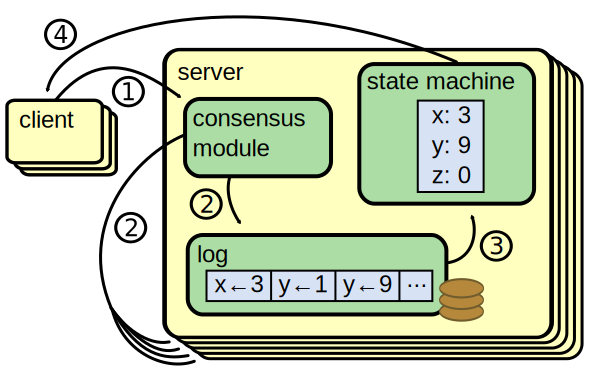
\includegraphics[scale=.50]{motivation/statemachine}
\vcaption[replicated state machine architecture]{
Replicated state machine architecture.
The consensus algorithm
manages a replicated log containing state machine commands from
clients. The state machines process identical sequences of commands
from the logs, so they produce the same outputs.}
\label{fig:motivation:statemachine}
\end{figure}

Replicated state machines are typically implemented using a replicated
log, as shown in Figure~\ref{fig:motivation:statemachine}. Each server stores a log
containing a series of commands, which its state machine executes in order.
Each log contains the same commands in the same order, so each state
machine processes the same sequence of commands. Since the state
machines are deterministic, each computes the same state and the same
sequence of outputs.

Keeping the replicated log consistent is the job of the consensus
algorithm. The consensus
module on a server receives commands from clients and adds them to its log.
It communicates with the consensus modules on other servers to
ensure that every log eventually contains
the same requests in the
same order, even if some servers fail. Once commands are properly
replicated, they are said to be \emph{committed}. Each server's state machine processes
committed commands in log order, and the outputs are returned to clients.
As a result, the servers appear to
form a single, highly reliable state machine.

Consensus algorithms for practical systems typically have the following
properties:
\begin{itemize}
\item They ensure \emph{safety} (never returning an incorrect
result) under all non-Byzantine
conditions, including network delays,
partitions, and packet loss, duplication, and reordering.
\item They are
fully functional (\emph{available}) as long as any majority of the servers are
operational and can communicate with each other and with clients.
Thus, a typical cluster of five servers can tolerate the
failure of any two servers.
Servers are assumed to fail by stopping; they may later recover from
state on stable storage and rejoin the cluster.
\item They do not depend on timing to ensure the consistency
of the logs: faulty clocks and extreme message delays can, at worst,
cause availability problems. That is, they maintain safety under an
\emph{asynchronous} model~\cite{Lynch:1996}, in
which messages and processors proceed at arbitrary speeds.
\item In the common
case, a command can complete as soon as a majority of the cluster
has responded to a single round of remote procedure calls; a minority
of slow servers need not impact overall system performance.
\end{itemize}


\section{Common use cases for replicated state machines}
\label{motivation:uses}

Replicated state machines are a general-purpose building block for making
systems fault-tolerant. They can be used in a variety of ways, and this
section discusses some typical usage patterns.

\begin{figure}
\hfill
\begin{subfigure}{.45\textwidth}
\centering
\includegraphics[scale=.5]{motivation/activeactive}
\caption{
The nodes in the cluster coordinate among themselves by reading from and
writing to the replicated state machine.
\\
}
\label{fig:motivation:activeactive}
\end{subfigure}
\hfill
\begin{subfigure}{.45\textwidth}
\centering
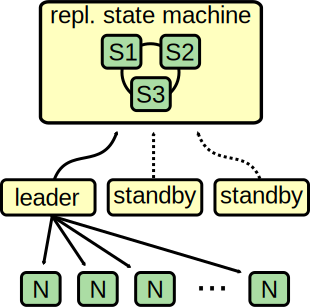
\includegraphics[scale=.5]{motivation/activepassive}
\caption{
One leader actively manages the nodes in the cluster and records its
state using the replicated state machine. Other standby servers are
passive until the leader fails.
}
\label{fig:motivation:activepassive}
\end{subfigure}
\hfill
\vcaption[common patterns for using a single replicated state machine]{
Common patterns for using a single replicated state machine.
}
\end{figure}


Most common deployments of consensus have just three or five servers
forming one replicated state machine. Other servers can then use this
state machine to coordinate their activities, as shown in
Figure~\ref{fig:motivation:activeactive}. These systems often use the
replicated state machine to provide
group membership, configuration management, or locks~\cite{Hunt:2010}.
As a more specific example, the replicated state machine could provide a
fault-tolerant work queue, and other servers could coordinate using the
replicated state machine to assign work to themselves.

A common simplification to this usage is shown in
Figure~\ref{fig:motivation:activepassive}. In this pattern, one
server acts as leader, managing the rest of the servers.
The leader stores its critical data in the consensus system.
In case it fails, other standby servers compete for the position of
leader, and if they succeed, they use the data in the consensus system
to continue operations.
Many large-scale storage systems that have a single cluster leader, such as
GFS~\cite{Ghemawat:2003}, HDFS~\cite{Shvachko:2010}, and
RAMCloud~\cite{Ousterhout:2011}, use this approach.

\begin{figure}
\centering
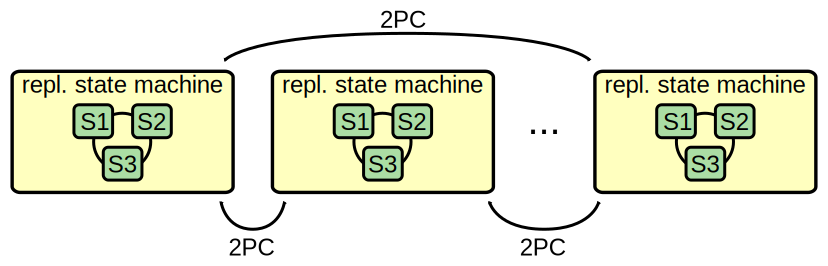
\includegraphics[scale=.5]{motivation/bigdata}
\vcaption[partitioned large-scale storage system using consensus]{
Partitioned large-scale storage system using consensus.
For scale, data is partitioned across many replicated state machines.
Operations that span partitions use a two-phase commit protocol.
}
\label{fig:motivation:bigdata}
\end{figure}

Consensus is also sometimes used to replicate very large amounts of
data, as shown in Figure~\ref{fig:motivation:bigdata}. Large storage
systems, such as Megastore~\cite{Baker:2011},
Spanner~\cite{Corbett:2012}, and Scatter~\cite{Glendenning:2011},
store too much data to fit in a single group
of servers. They partition their data across many replicated state machines,
and operations that span multiple partitions use a two-phase commit
protocol (2PC) to
maintain consistency.



\section{What's wrong with Paxos?}
\label{motivation:paxos}

\begin{figure*}
\centering
\includegraphics[scale=0.95]{motivation/paxossummary}
\vcaption[summary of the single-decree Paxos protocol]{
Summary of the single-decree Paxos consensus protocol.
See \cite{Lamport:2001} for a detailed explanation.
}
\label{fig:motivation:paxos:basic}
\end{figure*}


Over the last ten years, Leslie Lamport's Paxos protocol~\cite{Lamport:1998}
has become almost synonymous with consensus: it is the protocol
most commonly taught in courses, and most implementations of consensus
use it as a starting point. Paxos first defines a protocol capable
of reaching agreement on a single decision, such as a single replicated
log entry.  We refer to this subset as \emph{single-decree Paxos}.
Paxos then combines multiple instances of this protocol to facilitate
a series of decisions such as a log (\emph{Multi-Paxos}).
Single-decree Paxos is summarized in
Figure~\ref{fig:motivation:paxos:basic}, and Multi-Paxos is summarized
in Figure~\ref{fig:appendix:userstudy:paxossummary4}.
Paxos ensures safety and liveness (it eventually reaches consensus,
assuming an adequate failure detector
is used to avoid proposer livelock), and its correctness has been proven.
Multi-Paxos is efficient in the normal case, and Paxos supports changes
in cluster membership~\cite{Lorch:2006}.

Unfortunately, Paxos has two significant drawbacks.  The first drawback is
that Paxos is exceptionally difficult to understand. The full
explanation~\cite{Lamport:1998} is notoriously opaque; few
people succeed in understanding it, and only with great effort.
As a result, there have been several attempts to explain Paxos
in simpler terms~\cite{Lamport:2001, Lampson:1996, Lampson:2001}.
These explanations focus on the single-decree subset,
yet they are still challenging.
In an informal survey of attendees at NSDI 2012, we found few people who
were comfortable with Paxos, even among seasoned researchers.
We struggled with Paxos ourselves; we were not able to understand
the complete protocol
until after reading several explanations
and designing our own alternative protocol, a process that took
almost a year.

We hypothesize that Paxos' opaqueness stems from its choice of the
single-decree subset as its foundation. Single-decree
Paxos is dense and subtle: it is divided into two stages that do
not have simple intuitive explanations and cannot be understood
independently. Because of this, it is difficult to
develop intuitions about why the single-decree protocol works.
The composition rules for Multi-Paxos add significant additional
complexity and subtlety. We believe that the overall
problem of reaching consensus on multiple decisions (i.e., a log instead
of a single entry) can be decomposed in other ways that are more
direct and obvious.

The second problem with Paxos is that it does not provide a good
foundation
for building practical implementations. One reason is that
there is no widely agreed-upon algorithm for Multi-Paxos.
Lamport's descriptions are mostly about single-decree Paxos;
he sketched possible approaches to Multi-Paxos, but many
details are missing. There have been several attempts to flesh out and
optimize Paxos, such as \cite{Mazieres:2007}, \cite{Renesse:2011},
and \cite{Kirsch:2008},
but these differ from each other and from Lamport's sketches.
Systems such as Chubby~\cite{Chandra:2007} have implemented
Paxos-like algorithms, but in most cases their details have not been
published.


Furthermore, the Paxos
architecture is a poor one
for building practical systems; this
is another consequence of the
single-decree decomposition. For example, there is
little benefit to
choosing a collection of log entries independently and then melding
them into a sequential log; this just adds complexity.  It is simpler
and more efficient to design a system around a log, where new
entries are appended sequentially in a constrained order.
Another problem is that Paxos
uses a symmetric peer-to-peer approach at its core (though it
also suggests a weak form of leadership as a performance
optimization). This makes
sense in a simplified world where only one decision will be made,
but few practical systems use this approach. If a series of decisions
must be made, it is simpler and faster to first elect a
leader, then have the leader coordinate the decisions.
(Chapter~\ref{related} discusses Egalitarian Paxos, a recent
variant of Paxos that does not use a leader but in some situations can
be more efficient than algorithms that do; however, this algorithm is
much more complex than leader-based algorithms.)

As a result, practical systems bear little resemblance to Paxos.
Each implementation begins with Paxos, discovers the difficulties in
implementing it, and then develops a significantly different architecture.
This is time-consuming and error-prone, and the difficulties of
understanding Paxos exacerbate the problem.
Paxos' formulation may be a good one for proving theorems about
its correctness, but real implementations are so
different from Paxos that the proofs have little value. The following
comment from the Chubby implementers is typical:

{\defaultleftmargin{4em}{}{}{}
\begin{quote}
There are significant gaps between the description of the Paxos
algorithm and the needs of a real-world system\dots. the final system
will be based on an unproven protocol~\cite{Chandra:2007}.
\end{quote}
}

Because of these problems, we concluded that Paxos does not provide
a good foundation either for system building or for education.
Given the importance of consensus in large-scale software
systems, we decided to see if we could design an alternative consensus
algorithm with better properties than Paxos.  \name{} is the result
of that experiment.


%


